\chapter{SAFTools framework}
\label{chapter:framework}

% - diagram of whole system
% - table of supported SAF microarchitecture types, related primitives, and related RTL blocks, as well as relevant designs
% - Gating and merge with probably have no SL/Acc parsing support, possibly no case studies
% - Merge may only have RTL

Up to this point, everything we have discussed has been conceptual; this section will now introduce the SAFTools software framework, which implements the conceptual framework described in this work.

Prior sections introduce the conceptual framework in a bottom-up fashion, starting with RTL blocks and building up to high-level SAF microarchitecture blocks.

The natural workflow of the SAFTools framework runs in reverse: starting from a Sparseloop configuration file with declarative SAF specifications, SAFTools infers a SAF microarchitecture (Sections~\ref{chapter:primitive_taxo_model} and~\ref{chapter:saf_microarchitectures}), and then employs scale inference (Section~\ref{chapter:modeling}) in order to size the SAF microarchitecture primitives. The end result is a set of Accelergy models which hook into existing Sparseloop architectural buffer models in such a way, as to infer SAF microarchitecture action counts from architectural action counts.

Two YAML frameworks were developed for this work. \textit{Taxoscript} was developed to define SAF microarchitecture primitives and high-level SAF microarchitecture blocks. \textit{Modelscript} was developed to define SAF microarchitecture primitive analytical models.

\begin{figure}[H]
\centering
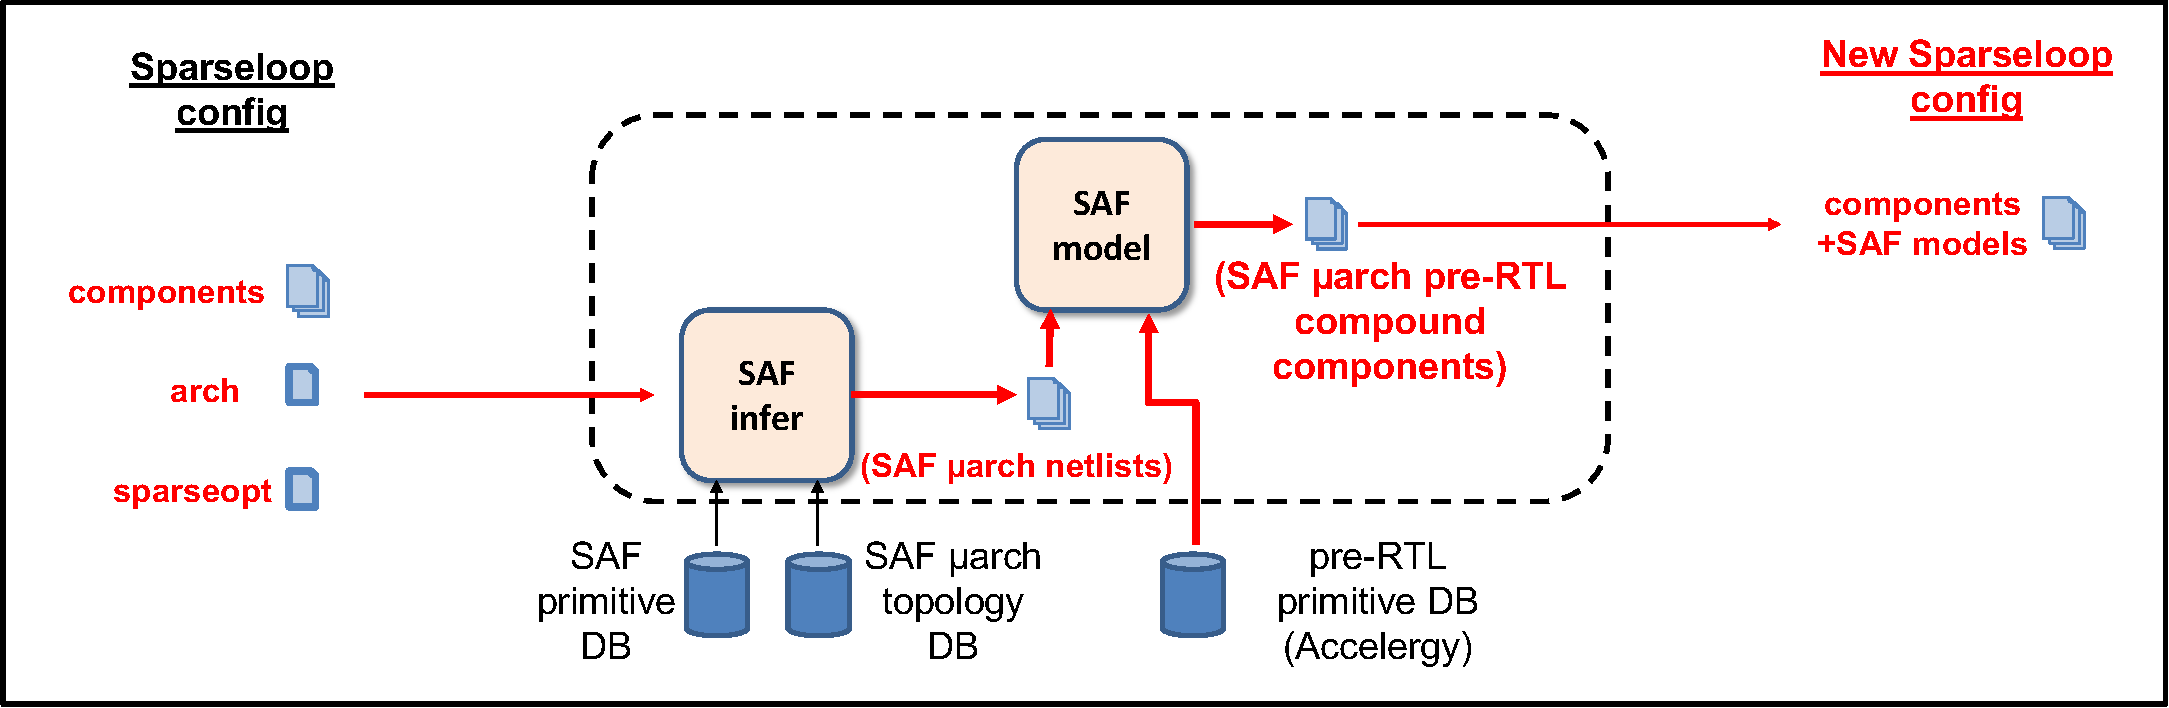
\includegraphics[width=0.5\textwidth]{figures/saftools_overview.pdf}
\caption{An overview of the SAFTools software suite.}
\label{fig:saftools_overview}
\end{figure}

\section{SAFinfer: SAF microarchitecture taxonomic inference}

SAFinfer is part of the SAFTool suite; it consumes the Sparseloop configuration file and applies \textit{taxonomic inference} in order to infer a SAF microarchitecture topology.

\subsection{Taxonomic inference}

Here, \textit{inferring} a SAF microarchitecture topology means

\begin{itemize}
\item Replacing declarative SAFs with high-level SAF microarchitecture blocks (i.e. FMT, SKIP) 
\item Solving for all attributes of the high-level SAF microarchitecture blocks, such that we have determined a particular customization for each high-level block.
\item Substituting in the appropriate SAF microarchitecture implementation topology (Section~\ref{chapter:saf_microarchitectures}) for each high-level SAF microarchitecture block, based on the customization.
\item Solving for all attributes of the SAf microarchitecture primitives within each implementation topology. This can be accomplished through (1) employing representation format or other surrounding design characteristics, to constraint the space of supported primitive customizations, or (2) allowing the user to specify free parameter values.
\end{itemize}

Notable, taxonomic inference does \textit{not} include scale inference: the result of taxonomic inference is a netlist of SAF microarchitecture components and the wires between them; no analytical models are produced, and scale parameters are still unspecified.

\subsection{Example}

A fully-worked example of taxonomic inference for an Eyeriss v2\cite{eyerissv2}-like design can found in Appendix\ref{appendix:safinfer_build}. Additionally the case-study in Section~\ref{chapter:case_studies} shows the result of taxonomic inference for a simple architecture with a bidirectional skipping SAF and CSR format SAFs.


\section{SAFmodel: primitive component scale inference and model export}

SAFmodel consumes the inferred SAF microarchitecture topology from SAFinfer, and applies \textit{scale inference} in order to infer optimized values for all SAF microarchitecture primitive scale parameters (Section~\ref{chapter:modeling}.

After performing scale inference, SAFmodel exports Accelergy models for the optimized SAF microarchitecture.

\subsection{Building the scale inference problem}

Recall that the output of SAfinfer is a netlist of SAF microarchitecture components. This netlist is hierarchical; the top level is the netlist connecting high-level SAF microarchitecture blocks (FMT, SKIP) to ``stubs'' which stand in for architectural buffers, and the bottom level is a netlist within each high-level block, which specifies the connectivity between primitives in the implementation topology.

SAFmodel first flattens this netlist, so that it contains only SAF microarchitecture primitives.

Next, SAFmodel implements the process of scale inference described in Section~\ref{chapter:modeling}: SAFmodel employes (1) workload boundary conditions and (2) primitive transfer relations, in order to infer the workload requirements imposed on each SAF microarchitecture primitive component.

This process yields a mixed-integer non-linear program (MINLP). SAFmodel attempts to solve this MINLP and minimize the total energy-per-action/area product of all primitive models, by tuning the scale parameters of the primitives within the feasible region imposed by the primitives' interface constraints.

\subsection{Accelergy model synthesis backend}

After solving the scale inference MINLP, SAFmodel synthesizes the following Accelergy primitive models:

\begin{itemize}
    \item \textit{SAF microarchitecture primitive models.} This primitive models are parameterized by the primitive scale parameters; the energy and area values associated with these models are derived from the characterized RTL blocks associated with the SAF microarchitecture primitive.
    \item \textit{High-level SAF microarchitecture block models.} No high-level block has its own energy/area model, however high-level blocks do lead to Accelergy \textit{compound component models}\cite{accelergy}, which compose primitive models in order to compute a compound energy-per-action and area value.
    \item \textit{Modified architectural buffer models.} SAFmodel scans the Accelergy configuration files for architectural buffer models; for each architectural buffer model it finds, it injects the high-level SAF microarchitecture block model(s) associated with buffer. This yields a set of modified architectural buffer models, in which each architectural action is formulaically coupled to high-level SAF microarchitecture block actions.
\end{itemize}

\subsubsection{The SAFmodel Accelergy estimator}

SAFmodel includes a custom Accelergy estimator\cite{accelergy}; this estimator comprehends the model format which is output by SAFmodel, thus facilitating integration of SAFmodel models into Accelergy.

\section{RTL block library}

% Overview of RTL support at time of writing

\subsection{45nm gate-level characterization}

Here, RTL ``characterization'' refers to simulation-modeling of the energy, area and timing-characteristics of small RTL designs, done for the purpose of creating analytical models (as opposed to for the purpose of designing a chip.)

The RTL blocks developed in this work were characteristized using Synopsys Design Compiler (SDC) to synthesize a gate-level netlist targeting the OpenPDK45 45nm PDK. The analytical models of RTL-block energy/area/latency reflect the SDC estimates of energy, area and timing characteristics (specifically propagation delay) based on the gate-level netlist.

It is noted that gate-level modeling of energy, area and especially timing may incur a relative accuracy penalty, since as observed by the authors of Wattch\cite{wattch}, ``Most existing power analysis tools achieve high accuracy by calculating power estimates for designs only after layout or floorplanning are complete...such tools are often quite slow, which compounds the difficulty of running them for a large space of design possibilities.'' Being that the RTL library comprises a only a portion of this work, the much faster gate-level modeling process was favored to facilitate short turnaround time during the RTL development process. Even using gate-level synthesis and modeling, it was still time-consuming to characterize highly parallel RTL blocks with deep vector pipelines. 

Improving modeling accuracy by performing modeling after the floorplanning or layout phases could be a valuable task for future research.

\subsection{RTL development in Chisel}

Early on, it was decided to develop the RTL blocks in a higher-level language than Verilog. While Verilog supports parameterization, higher-level languages provide more powerful and concise abstractions for designing parameterized RTL. 

Since SDC takes Verilog-language RTL as input, any workflow for defining the RTL blocks had to ultimately produce Verilog.

The following high-level HDLs and workflows were considered as candidates for implementing the RTL library in this work:

\begin{itemize}
    \item SystemC\cite{systemc}\footnote{SystemC language homepage: \url{https://systemc.org/}}, a C++ framework for transaction-level modeling (TLM)\cite{systemc}, which decouples implementation from communication. Intel\textregistered Compiler for SystemC \footnote{\url{https://github.com/intel/systemc-compiler}} can synthesize SystemVerilog from SystemC. SystemC was ultimately discarded as an option due to the difficulty in automatically converting the SystemVerilog to Verilog that was acceptable by SDC.
    \item Bluespec SystemVerilog\cite{bluespec}\footnote{Bluespec language homepage: \url{https://github.com/B-Lang-org/bsc}}, a very high-level HDL with an open-source compiler, support for software-like syntax for parameterized component design, and a workflow that exports to Verilog.
    \item Chisel\cite{chisel}\footnote{Chisel language homepage: \url{https://www.chisel-lang.org/}}, a hardware description language (HDL) implemented as a Scala framework, which was developed by the Berkeley Architecture Research (BAR) Group\footnote{U.C. Berkeley Architecture Research Group: \url{https://bar.eecs.berkeley.edu/}}. Similar to Bluespec, is a very high-level language with an open-source compiler, support for software-like syntax for parameterized component design, and a workflow that exports to Verilog.
\end{itemize}

Between Bluespec and Chisel, ultimately Chisel was selected as it was the most intuitive and is very widely-used within the computer-architecture community.